\documentclass[tikz,border=12pt]{standalone}
\usepackage{newtxtext}
\usetikzlibrary{arrows.meta,positioning,shapes.geometric,fit,calc}
\definecolor{navy}{HTML}{173B70}
\definecolor{bluefill}{HTML}{EAF2FB}
\definecolor{greenfill}{HTML}{EAF7EF}
\definecolor{amberfill}{HTML}{FFF4DD}
\definecolor{redfill}{HTML}{FDECEC}
\tikzset{
  flow/.style={draw=navy,thick,rounded corners=3pt,fill=bluefill,
    align=center,font=\sffamily\small,minimum height=9mm,minimum width=29mm},
  action/.style={flow,fill=greenfill},
  decision/.style={diamond,draw=navy,thick,fill=amberfill,align=center,
    font=\sffamily\scriptsize,aspect=2.1,inner sep=1.5pt},
  review/.style={flow,fill=redfill},
  group/.style={draw=black!55,dashed,rounded corners=4pt,inner sep=5pt},
  arrow/.style={-{Stealth[length=2.4mm]},thick,draw=black!75},
  note/.style={font=\sffamily\scriptsize,text=black!70,align=center}
}
\begin{document}
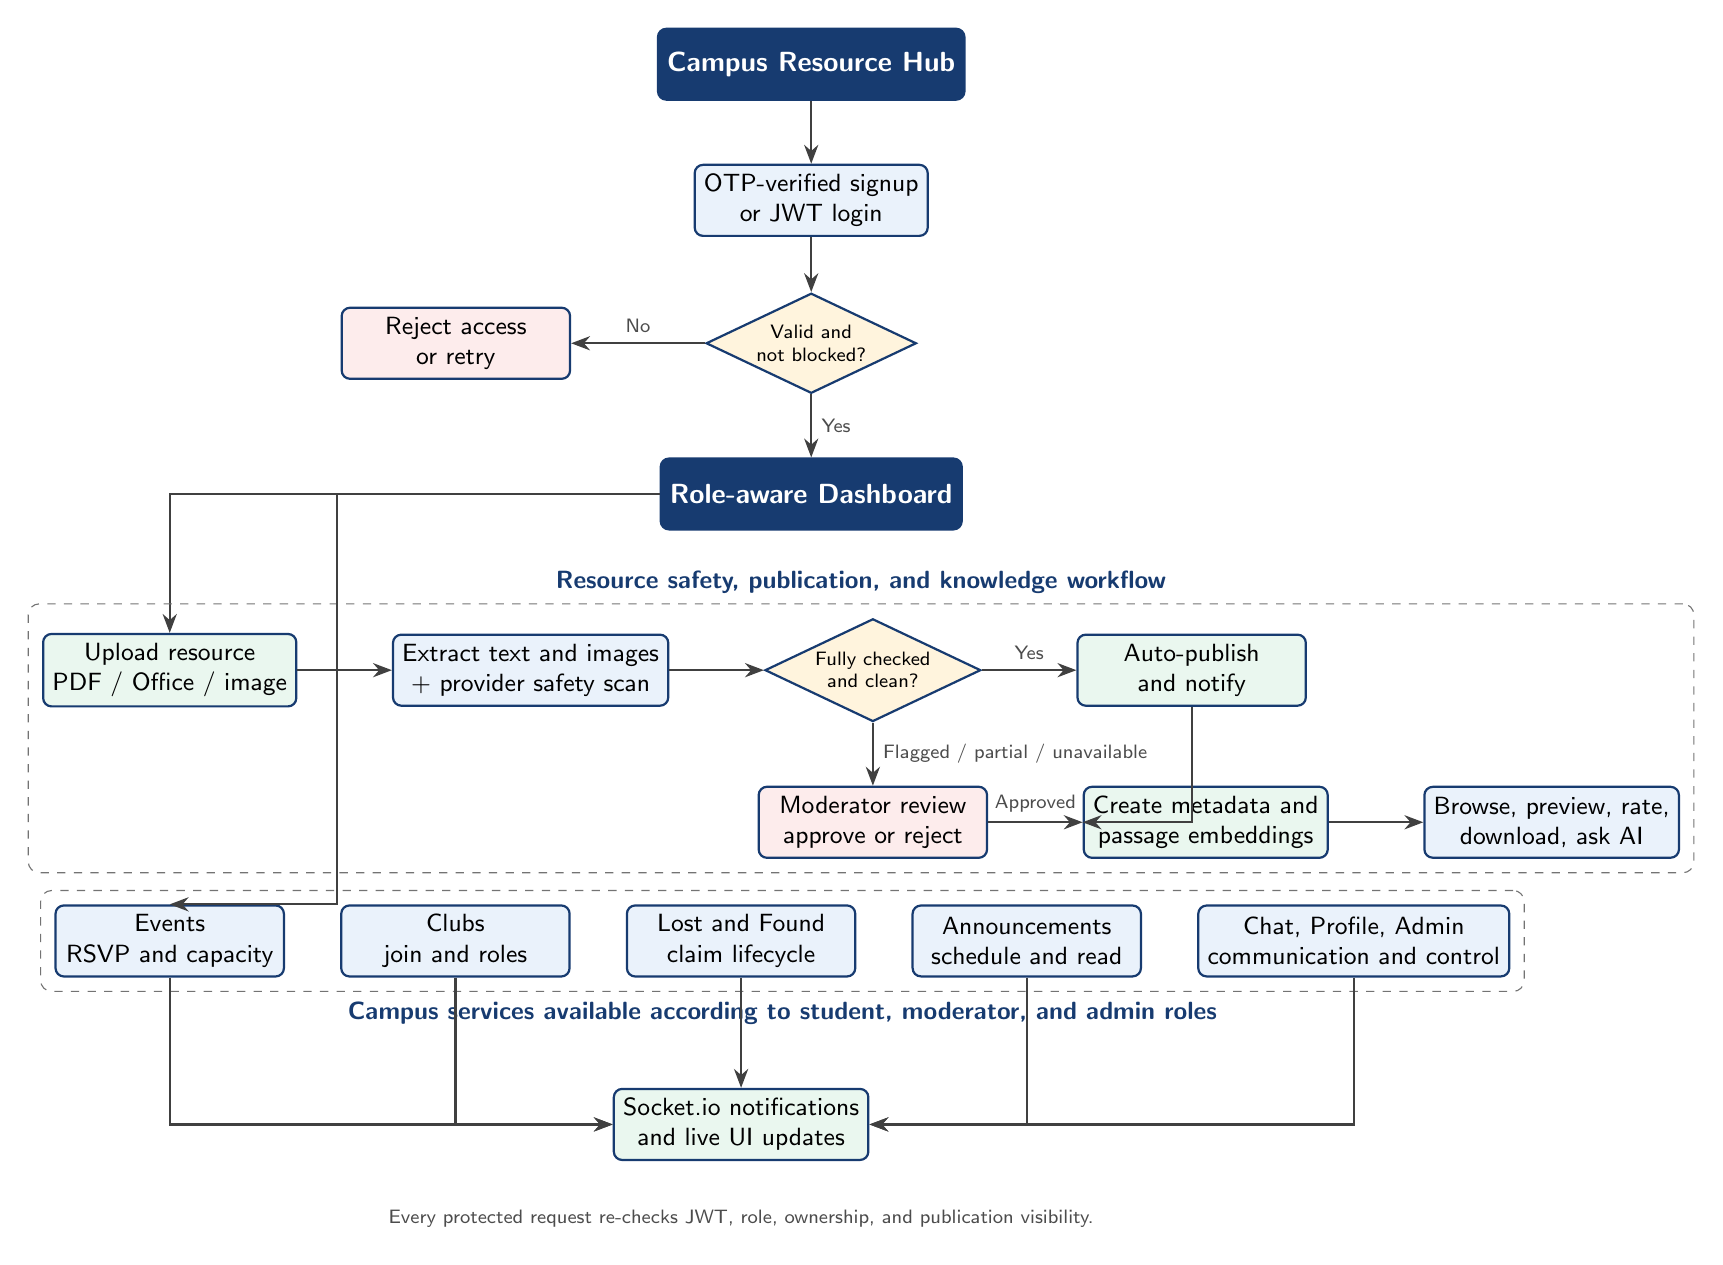
\begin{tikzpicture}[node distance=8mm and 12mm]
  \node[flow,fill=navy,text=white,font=\sffamily\bfseries] (entry) {Campus Resource Hub};
  \node[flow,below=of entry] (auth) {OTP-verified signup\\or JWT login};
  \node[decision,below=7mm of auth] (valid) {Valid and\\not blocked?};
  \node[review,left=17mm of valid] (deny) {Reject access\\or retry};
  \node[flow,fill=navy,text=white,font=\sffamily\bfseries,below=8mm of valid] (dash) {Role-aware Dashboard};

  \draw[arrow] (entry) -- (auth);
  \draw[arrow] (auth) -- (valid);
  \draw[arrow] (valid) -- node[note,above]{No} (deny);
  \draw[arrow] (valid) -- node[note,right]{Yes} (dash);

  \node[action,below left=13mm and 46mm of dash] (upload) {Upload resource\\PDF / Office / image};
  \node[flow,right=of upload] (extract) {Extract text and images\\+ provider safety scan};
  \node[decision,right=of extract] (safe) {Fully checked\\and clean?};
  \node[action,right=of safe] (publish) {Auto-publish\\and notify};
  \node[review,below=8mm of safe] (queue) {Moderator review\\approve or reject};
  \node[action,right=of queue] (index) {Create metadata and\\passage embeddings};
  \node[flow,right=of index] (discover) {Browse, preview, rate,\\download, ask AI};

  \draw[arrow] (dash) -| (upload);
  \draw[arrow] (upload) -- (extract);
  \draw[arrow] (extract) -- (safe);
  \draw[arrow] (safe) -- node[note,above]{Yes} (publish);
  \draw[arrow] (safe) -- node[note,right]{Flagged / partial / unavailable} (queue);
  \draw[arrow] (queue) -- node[note,above]{Approved} (index);
  \draw[arrow] (publish) |- (index);
  \draw[arrow] (index) -- (discover);

  \node[group,fit=(upload)(extract)(safe)(publish)(queue)(index)(discover),
    label={[font=\sffamily\bfseries\small,text=navy]above:Resource safety, publication, and knowledge workflow}] {};

  \node[flow,below=25mm of upload] (events) {Events\\RSVP and capacity};
  \node[flow,right=7mm of events] (clubs) {Clubs\\join and roles};
  \node[flow,right=7mm of clubs] (lost) {Lost and Found\\claim lifecycle};
  \node[flow,right=7mm of lost] (announce) {Announcements\\schedule and read};
  \node[flow,right=7mm of announce] (chat) {Chat, Profile, Admin\\communication and control};

  \draw[arrow] (dash.west) -- ++(-41mm,0) |- (events.north);

  \node[group,fit=(events)(clubs)(lost)(announce)(chat),
    label={[font=\sffamily\bfseries\small,text=navy]below:Campus services available according to student, moderator, and admin roles}] {};

  \node[action,below=14mm of lost] (notify) {Socket.io notifications\\and live UI updates};
  \draw[arrow] (events) |- (notify);
  \draw[arrow] (clubs) |- (notify);
  \draw[arrow] (lost) -- (notify);
  \draw[arrow] (announce) |- (notify);
  \draw[arrow] (chat) |- (notify);

  \node[note,below=5mm of notify] {Every protected request re-checks JWT, role, ownership, and publication visibility.};
\end{tikzpicture}
\end{document}
